
\pagebreak
\section{Curve Fitting}

\subsection{Fit}
The base Matlab install only has some rudimentary polynominal curve fitting.
 Since you're likely to encounter more complicated curve fitting, this section is dependent on the curve-fitting toolbox.

\begin{quote}
\verbatiminput{code/ch09_fit.m}
\end{quote}

You can also interactively fit data with the "cftool" command.

\begin{figure}[ht!]
\centering
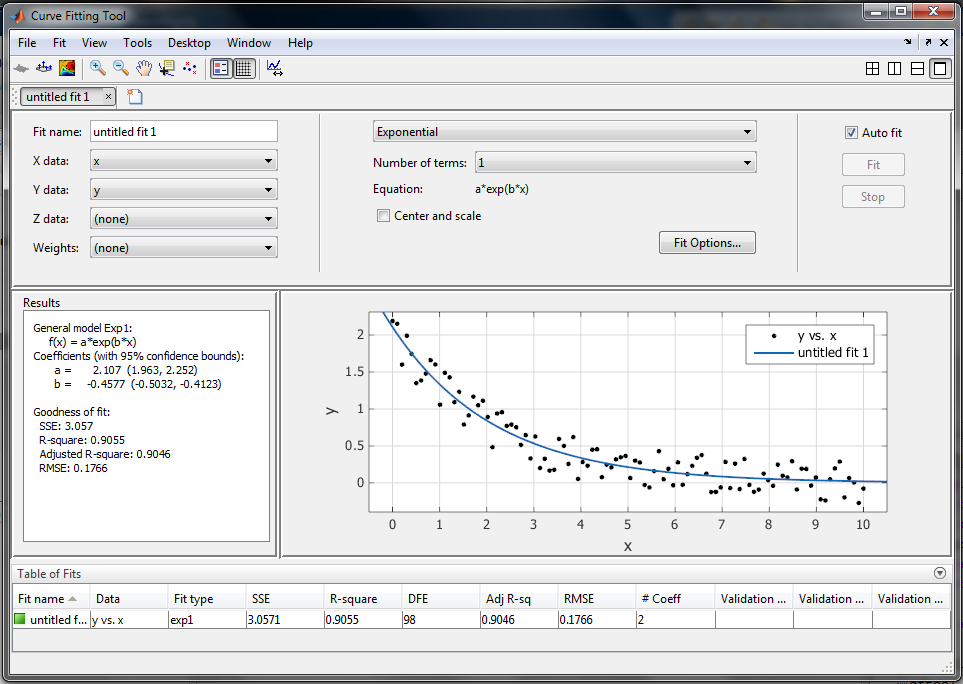
\includegraphics[width=120mm]{img/cftool.png}
\caption{cftool. From here you can load and fit data.}
\label{guiload}
\end{figure}

\pagebreak
\subsection{Custom Fit}
Quite often, you have your own model to fit to the data.
 You can use that for the fit, but we have to construct the model first.
 Once you have a model, we give the fitting routine bounds for the variables and initial guesses.

\begin{quote}
 \verbatiminput{code/ch09_customfit.m}
\end{quote}

\pagebreak
\subsection{Confidence Intervals}
Once you have your data fit, we can find out well the parameters are fit by using confidence intervals.

\begin{quote}
 \verbatiminput{code/ch09_confint.m}
\end{quote}
